\documentclass[titlepage]{article}                %% What type of document you're writing.

%%%%% Preamble

%% Packages to use

\usepackage{verbatim}        %% Display text verbatim
\usepackage{url}        %% Special commands for URLs
\usepackage{amsmath,amsfonts,amssymb}        %% AMS mathematics macros
\usepackage{graphicx}        %% Commands for including graphics

\usepackage{amsthm}	%% required for theorem and proof environments

\usepackage[en-AU]{datetime2}  %% Change date formats

%% Set up environments for theorems, lemmas, and corollaries using the amsthm package.
%% Use the default plain theorem style.

%% \theoremstyle{plain}		%% Default theorem style
\newtheorem{theorem}{Theorem}
\newtheorem{lemma}{Lemma}
%% \newtheorem{corollary}{Corollary}
%% \newtheorem{proposition}{Proposition}

%% Set up environments for definitions and examples using the amsthm package.
%% These use a theorem style different from the default plain theorem style.

\theoremstyle{definition}
\newtheorem{definition}{Definition}
%% \newtheorem{example}{Example}

%% Set up environments for remarks and notes using the amsthm package.
%% These use another theorem style different from the default plain theorem style.

\theoremstyle{remark}
\newtheorem{remark}{Remark}
%% \newtheorem{note}{Note}

%% Redefine QED symbol to be solid box.

%% \renewcommand{\qedsymbol}{\rule{0.6em}{0.675em}}


%% Title Information.  This may come in the document before the \maketitle
%%  command.

\title{Basic \LaTeX{} Typesetting}
\author{William J. Turner}
%% \date{2 July 2004}                %% By default, LaTeX uses the current date

%%%%% The Document

\begin{document}

\maketitle

\begin{abstract}
This paper is a short introduction to using \LaTeX{} at Wabash College.  It
introduces the basics of a \LaTeX{} document.
\end{abstract}

\tableofcontents

\clearpage

\section{Introduction}
\label{intro}

Have you ever tried to write a mathematical paper in Microsoft Word?  Newer
versions of Word contain an equation editor that makes it possible, but you
probably find moving the mouse to click on each symbol annoying and tedious.
Don't despair; there's another way!

\LaTeX{} is the standard tool to typeset papers in mathematics, physics,
economics, and other disciplines.  It is so common that most scientific and
mathematical journals give special instructions on how to format articles for
submission.  In fact, it is very hard to find a mathematical journal that does
not explicitly prefer \LaTeX{} submissions over any other type of electronic
submission.

\LaTeX{} is actually not a program.  It is a set of macros for Donald Knuth's
\TeX{} typesetting program, which takes a plain text file encoded with special
commands and outputs a typeset document.  Some people prefer to use plain
\TeX{}, but we will concentrate on \LaTeX{} for its widespread use and ease of
learning.

Because \LaTeX{} uses just plain text files, you will use the keyboard to
input everything.  You might find this more difficult at first to remember all
the commands, but eventually you will find it much faster to write a
mathematical paper using \LaTeX{} than Microsoft Word.

The best way to learn \LaTeX{} is to experiment.  Take a file that already
works and change it and see what happens.  Use this document or any \LaTeX{}
document you find on the web.  You can even start from scratch.

Throughout this paper, we describe the various parts of this document.
Section~\ref{start} describes how to get started on Wabash's public Windows
machines, and Section~\ref{basic} describes basic \LaTeX{} files and commands.
Sections \ref{mathematics} and \ref{advanced} describe how to typeset
mathematical equations and how to incorporate more advanced environments such
as automatic references, graphics, and floating figures and tables.  Finally,
since we have only scratched the surface of \LaTeX{}'s capabilities,
Section~\ref{more} describes how to find more information.

\section{Getting Started}
\label{start}

To begin, you need only a few programs: a basic text editor and a \LaTeX{}
processor.  On a Unix machine, one often runs these separately.  For example,
you could run an editor such as emacs or vi to edit the file and then run the
command \verb=latex= to process the file.  You will find most \LaTeX{}
documentation describing this method.  Because it is so widely described, and
because you will likely use a public Windows machine to typeset your document,
we will concentrate on the two integrated development environments (IDEs)
installed on all public PCs on campus: PCTeX and ProTeXt.  Section~\ref{more}
describes a website where you can find links to other free and commercial
versions of \LaTeX{} for any platform.

\subsection{PCTeX}

Wabash College has a site license for the commercial software PCTeX.  You can
find it on the public Windows machines under mathematics software.  You can
also buy a personal copy from the website \url{http://www.pctex.com}, or you
can get a copy to evaluate free for 30 days.  This might be a good way to use
\LaTeX{} on your personal computer in the short term.

Once you start the program, it acts like most standard Windows applications.
You can use the \emph{File} menu in the upper left to open \LaTeX{} files.
PCTeX comes with several sample files in a directory named \emph{samples}.
The public machines may open to it automatically.  If not, look for a
directory named \emph{PCTeX} on the local drive.  The \emph{samples} directory
will be in it, probably a level or two down.

After you have opened a \LaTeX{} file, or have created your own, you can
typeset it with the \emph{Typeset} button in the middle of the row below the
menus near the top of the window.  Be sure you see \emph{\LaTeX{}} in the
pull-down menu next to it.  It might not be activated yet.  In which case, you
need to go to the \emph{Typeset} menu and run \emph{INITeX}.  Choose the
\LaTeX{} macros and then run \emph{INITeX}.  

By typesetting your document, you create a file called a \emph{DVI} file that
is independent of the printer you will use.  This file should appear, and you
can see the results of your efforts.  You may encounter error in typesetting
your document.  For example, we often find misspelled commands that \LaTeX{}
doesn't understand.  Fortunately, PCTeX will tell us where it encounters
errors so we can fix them.

You might also have to typeset the program a second time.  This often happens
when you are using \LaTeX{}'s automatic referencing capabilities.  If PCTeX
suggests you typeset the document again, you should do it.

Once you successfully typeset your program and create a DVI file, you can
print it or you can export it to various document types.  If you want to send
it to someone else, we suggest exporting it as a PDF file by using the
\emph{Export} command in the \emph{File} menu.

%\subsection{ProTeXt}
%
%Wabash College also installed a copy of the free software ProTeXt on all
%public PCs.  In particular, the public machines have the TeXnicCenter IDE
%installed.  You can find it on the public Windows machines under mathematics
%software: 
%\begin{center}
%Start / Courses / Mathematics / ProTeXt / TeXnicCenter .
%\end{center}
%You can also download a personal copy from the website
%\url{http://www.tug.org}.  This may be your best long-term way to use \LaTeX{}
%on your personal computer.
%
%Once you start the program, it acts like most standard Windows applications.
%You can use the \emph{File} menu in the upper left to open \LaTeX{} files.
%TeXnicCenter does not appear to come with any sample files, but you can use
%the samples from PCTeX or any other \LaTeX{} files.
%
%After you have opened a \LaTeX{} file, or have created your own, you can
%typeset it with the click of a button.  Look for a pull-down menu in the
%middle of the row below the menus near the top of the window.  It will
%probably say \verb|LaTeX => PDF|.  (It may also say \verb|LaTeX => DVI| or
%\verb|LaTeX => PS|.)  This tells TeXnicCenter what format to make the output.
%If it does not say PDF, you may want to change it to PDF.  Any of the formats
%should work, but PDF is a bit more universal.
%
%Two buttons to the right of this pull down menu, you will see a button with an
%arrow pointing downward to a stack of papers.  This button will create the
%output.  Push it when you want to create your PDF file.
%
%Another two buttons to the right is a button with a paper and a magnifying
%glass.  Pushing this button opens the viewer to view your output file.
%Alternatively, another two buttons to the right you will see a button that is
%a combination of these two buttons.  This button both creates the output and
%opens the viewer.
%
%You may encounter error in typesetting your document.  For example, we often
%find misspelled commands that \LaTeX{} doesn't understand.  Fortunately,
%TeXnicCenter will tell us where it encounters errors so we can fix them.
%Notice the log at the bottom of the screen.  At the very end, it should tell
%you how many errors and warnings it encountered.  Errors will keep your
%document from compiling, while warnings will make it appear incorrectly.  You
%must fix errors, but you can ignore warnings if you do not care about the
%appearance.  You can scroll back up through the log to see what happened.
%Look for the colorful symbols on the left side that mark warnings and errors.
%
%You might also have to typeset the program a second time.  This often happens
%when you are using \LaTeX{}'s automatic referencing capabilities.
%Unfortunately, TeXnicCenter is not as good as PCTeX at suggesting you typeset
%the document again.  TeXnicCenter will mark each undefined reference with a
%warning, and the last warning in the log should tell you if you need to
%typeset the document again.  You may also notice an unusually large number of
%warnings when you have undefined references.  You may want to get in the habit
%of typesetting it two or three times, especially when you are preparing the
%final version.

\subsection{TeXworks}

Wabash College also installed a copy of the free software TeXworks on all
public PCs.  You can find it on the public Windows machines under mathematics
software: 
\begin{center}
Start / Courses / Mathematics / TeXworks .
\end{center}
You can also download a personal copy from the website
\url{http://www.tug.org}.  This may be your best long-term way to use \LaTeX{}
on your personal computer.

Once you start the program, it acts like most standard Windows applications.
You can use the \emph{File} menu in the upper left to open \LaTeX{} files.
You can use the "New from Templates" entry in the \emph{File} menu to open templates or sample files.

After you have opened a \LaTeX{} file, or have created your own, you can
typeset it with the click of a button.  Look for the \emph{Typeset} menu in the
middle of the menus near the top of the window.  When you open the menu, you can choose which program(s) you want to use to create the output.  It will
probably default to \emph{pdfLaTeX+MakeIndex+BibTex}.  I suggest you either use that or \emph{pdfLaTeX}.

You may encounter error in typesetting your document.  For example, we often
find misspelled commands that \LaTeX{} doesn't understand.  Fortunately,
TeXworks will tell us where it encounters errors so we can fix them.
Notice the log at the bottom of the screen.  At the very end, it should tell
you how many errors and warnings it encountered.  Errors will keep your
document from compiling, while warnings will make it appear incorrectly.  You
must fix errors, but you can ignore warnings if you do not care about the
appearance.  You can scroll back up through the log to see what happened.

You might also have to typeset the program a second time.  This often happens
when you are using \LaTeX{}'s automatic referencing capabilities.
TeXworks will often automatically typeset the document a second time, but if you find any undefined references---which will be marked by ``??''--you might first try typesetting it again.

\subsection{\LaTeX{} on Your Personal Computer}

You can also use \LaTeX{} on your personal computer.  The \TeX{} Users Group
website~\cite{tug} contains information on many commercial and free \TeX{} and
\LaTeX{} implementations for all operating systems.  If you have a PC, you can
install a demo version of PCTeX on your computer, or you can other free
versions such as ProTeXt, TeX Live, fpTeX, emTeX, or MikTeX.  On a Windows machine, I I suggest you install the latest version version of MikTeX, which should come with TeXworks.  (You might also want to install Ghostscript and GSView to view postscript files.)  On a Mac, my
colleagues in the Physics Department suggest TeXShop., which is very similar to TeXworks.  You can find its
website by searching on Google.

\subsection{\LaTeX{} Online}

It is becoming increasingly more popular to use \LaTeX{} online.  Overleaf is an online, collaboarative \LaTeX{} editor that is available for free for students.  It also has more advanced memberships with more features for a monthly or annual fee.  You can find it here: \url{https://www.overleaf.com/}.  It also has documentation to help you learn \LaTeX{} at \url{https://www.overleaf.com/learn}.

Overleaf may act a little differently from the other compilers I mentioned above.  In particular, students have told me the behavior of the Q.E.D. symbol differs from what I describe in Section~\ref{subsec: proofs}, and that the \verb|\qedhere| command is not supported.


In order to submit an assignment that you write in Overleaf, you will probably need to download the output or possibly the source file.  You can download either of them by clicking on the \verb|Menu| button at the top left of the proejct screen.  The source files will be in a zipper file, which you may need to extract.  The output should be in a single PDF file.

\section{Basic \LaTeX}
\label{basic}

\subsection{Commands and Comments}
\label{sec: comments}

As you look at any \LaTeX{} file, you will see various funny-looking strings
of letters.  In several places, you will see the character \verb=%=.  This
signifies the rest of the line is a comment, which \LaTeX{} will ignore.  You
can use comments to take out statements you no longer want, or to document
your work.

\LaTeX{} commands begin with the character \verb=\= and run until the first
whitespace.  Some commands require arguments, such as the
\verb=\documentclass{...}= command that begins the file.  Other commands, such
as \verb=\maketitle= require no arguments.  For example, we can print the
special word \LaTeX{} with the command \verb=\LaTeX=.  However, \LaTeX{}
recognizes the whitespace after the command as ending the command, not as
space between words.  Notice there is no space after the word \LaTeX in this
sentence.  For this reason, we use the braces \verb={= and \verb=}= to keep
the command and the whitespace separate.  Notice, throughout the file we use
the command \verb=\LaTeX{}=.  We could have also used the command
\verb={\LaTeX}= to achieve the same result.


\subsection{File Layout}

Every \LaTeX{} file consists of two parts: the preamble and the body.  The
\emph{preamble} begins with the \verb=\documentclass=, usually the first line
of the file, and sets certain information about the document.  In this case,
the command 
\begin{verbatim}
        \documentclass{article}
\end{verbatim}
says we are writing an article.  The command also may take options.  For
example, we could use the command \verb=\documentclass[12pt]{...}= to indicate
a 12 point font, or \verb=\documentclass[10pt,a4paper]{...}= to indicate 10
point font on A4 paper.  We could have also used \verb=\documentclass{report}=
to create a report or \verb=\documentclass{book}= to create a book.  Different
document classes behave differently.  We will concentrate on the article class
here.  Our preamble also includes commands to use additional packages.

The \emph{body} begins with the command \verb=\begin{document}= and ends with
the command \verb=\end{document}=, and it contains all the text of the
document.  \LaTeX{} will ignore anything after the \verb=\end{document}=
command.


\subsection{Titles, Authors, Dates}

The command \verb=\maketitle= that appears near the beginning of the body of
our file tells \LaTeX{} to make the title for the document.  It uses
information that we input in commands \verb=\title{...}=, \verb=\author{...}=,
and possibly \verb=\date{...}= sometime before the \verb=\maketitle= command.
We placed these commands in the preamble, but we could have just as easily
placed them in the body before the \verb=\maketitle= command.

\LaTeX{} requires us to use two of these commands: namely \verb=\title{...}=
and \verb=\author{...}=.  The \verb=\date{...}= is special because \LaTeX{}
will use today's date if we don't specify a date.  You might not specify a
date so \LaTeX{} will tell you the date you last \LaTeX{}ed the file, or you
might want to specify the date so \LaTeX{} will not change it on you.

\subsection{Sections}

You can divide a \LaTeX{} document into sections using the
\verb=\section{...}= command.  This command automatically numbers the sections
using an internal counter.  \LaTeX{} also has other sectioning commands to produce other levels of
headings.  Descending for \verb=\section{...}=, \LaTeX{} also has the commands
\begin{verbatim}
        \subsection{...}
        \subsubsection{...}
        \paragraph{...}
        \subparagraph{...}
\end{verbatim}
for increasingly finer divisions.  
        
Each of these sectioning commands also has an unnumbered version
\begin{verbatim}
        \section*{...}
        \subsection*{...}
        \subsubsection*{...}
        \paragraph*{...}
        \subparagraph*{...}
\end{verbatim}
These commands produces the same heading style without a counter.  For
example, the References section after Section~\ref{more} is produced with in
this way, although the mechanism is actually hidden within the
\verb=\bibliography{...}= command.  You might find this useful for typesetting
your homework where you might not want the section numbers to appear.

\LaTeX{} also has a \verb=\part= command that lies above the
\verb=\section= command in this hierarchy.  The book and report classes
also have a \verb=\chapter= command between parts and sections.

This automatic numbering is helpful when you rearrange sections.  It is also
useful when you want to automatically reference a section as described in
Section~\ref{bib}.  You can also create a table of contents, although you will
probably not encounter that in a paper.

\subsection{Words, Paragraphs, and Whitespace}

\LaTeX{} interprets \emph{blank spaces}, \emph{tabs}, and \emph{carriage
returns} as the end of words and commands.  It does not matter how many spaces
or tabs you put between words or commands.  \LaTeX{} will ignore this when it
places the space between words in the final output.  This means you can leave
whitespace (for example through indenting a line) only for your own
convenience.

\LaTeX{} interprets one or more \emph{empty lines} as the end of a paragraph.  
Once again, the spacing between paragraphs is independent of the number of
empty lines.  However, you can only leave a blank line if you want to start a
new paragraph.  If you want to leave a blank line for your convenience without
starting a new paragraph, you can cheat by making the line contain a blank
comment by starting it with a comment character \verb=%=.  (See
Section~\ref{sec: comments}.)

\LaTeX{} treats each paragraph as one long string of words.  It
then breaks up lines automatically independent of the input, and makes the
spacing between the words on each line as uniform as possible so that each
line is left and right justified.  It will also automatically space and indent
each paragraph based upon the document class in use.


\subsection{Quotation Marks}

Another trick you might encounter is placing quotation marks around a
sentence.  \LaTeX{} recognizes a difference between \verb='= and \verb=`=, and
it usually interprets \verb="= as \verb=''=.  The make the quotation marks
appear normally, use \verb=``= and \verb=''= to quote material.  For example,
\verb=``this''= produces ``this.''

\subsection{Tables}

Sometimes you might want to put information in a table.  To do so, you can use
the \emph{tabular} environment.  For example, the text
\begin{verbatim}
        \begin{tabular}{lccr}
                Name & Test 1 & Test 2 & Average \\
                Bob & 90 & 80 & 85 \\
                Joe & 60 & 90 & 75
        \end{tabular}
\end{verbatim}
produces the table

\begin{tabular}{lccr}
        Name & Test 1 & Test 2 & Average \\
        Bob & 90 & 80 & 85 \\
        Joe & 60 & 90 & 75
\end{tabular}

Be sure to leave a blank line before and after the environment so it doesn't
place the table inside a paragraph.

Here the command \verb$\begin{tabular}{lccr}$ begins the \emph{tabular}
environment and tells \LaTeX{} to make the table have four columns.  The
\verb={lccr}= says first one is left-justified, the middle two are centered,
and the last is right-justified.  The command \verb$\end{tabular}$ ends the
\emph{tabular} environment.  Between these two commands, we place the body of
the matrix in a \emph{row-major} form where we read across each row before
going to the next row.  We separate the entries of each row with ampersands \&
and separate each line with the newline command \verb$\\$. 

We can also place vertical and horizontal lines between the rows and columns
of the table.  We place vertical lines between the columns by placing a
\verb=|= between the justification indicators at the beginning of the
environment.  We place horizontal lines between the rows by using the
\verb=\hline= command.  This command must come one a new line, so be sure to
end any line before it with the newline command \verb=\\=.  For example,  the
text
\begin{verbatim}
        \begin{tabular}{||l|c|c|r||}
                \hline
                \hline
                Name & Test 1 & Test 2 & Average \\
                \hline
                Bob & 90 & 80 & 85 \\
                Joe & 60 & 90 & 75 \\
                \hline
                \hline
        \end{tabular}
\end{verbatim}
produces the table

\begin{tabular}{||l|c|c|r||}
        \hline
        \hline
        Name & Test 1 & Test 2 & Average \\
        \hline
        Bob & 90 & 80 & 85 \\
        Joe & 60 & 90 & 75 \\
        \hline
        \hline
\end{tabular}

\section{Mathematics}
\label{mathematics}

\LaTeX{} handles mathematical equations with ease.  You enter mathematical
equations by switching to \emph{math} mode.

\subsection{Text and Display Styles}

\LaTeX{} has type types of mathematical equations: \emph{text} and
\emph{display} styles.  \LaTeX{} changes slightly how equations are displayed
depending on the style, but you enter mathematics the same way in both.

You can enter equations in text style to occur in the line of the text by
placing a dollar sign \$ on either side.  For example, \verb/$x + y = z$/
produces $x + y = z$.  You can also enter equations in display style to occur
centered on their own line by placing two dollar signs \$\$ on either side.
For example, \verb/$$x + y = z$$/ produces $$x + y = z$$

\subsection{AMS \LaTeX}

The American Mathematical Society created additional \LaTeX{} macros to make
typesetting mathematical equations even easier \cite{amslatex}.  In this
document, we are using the \texttt{amsmath}, \texttt{amsfont}, and \texttt{amssymb}
packages.  The manual for the \texttt{amsmath} package \cite{amsldoc} describes
more features of this package than we will go into here.  In particular, you
might be interested in how to number equations, how to split equations over
several lines in display mode, or how to create new mathematical operators
such as $\sin$.  The AMS also created a short guide to typesetting mathematics
with these three packages \cite{ams-guide}.

The AMS also has a fourth package, \texttt{amsthm}, that you can use to typeset
theorems and proofs \cite{amsthm}.  You might find these features more useful
in theory classes and when writing research papers.  See Section~\ref{sec:
theorems} for more information.

\subsection{Superscripts and Subscripts}
\label{scripts}

To enter a superscript such as in an exponent, you use the \verb$^$ character.
For example, \verb$e^x$ produces $e^x$.  To use more complicate exponents, you
must group the exponent with braces.  For example, \verb$e^{x+1}$ produces
$e^{x+1}$.

Similarly you can enter subscripts with the \verb$_$ character.  For example,
\verb$x_0$ produces $x_0$, and \verb$x_{i+3}$ produces $x_{i+3}$.

\subsection{Binary Relations and Negations}

We can compare two mathematical quantities by connecting them with a relation
such as $=$, $\leq$, or $\propto$.  Table~\ref{tab:binary} in
Appendix~\ref{symbols} lists several common binary operators and relations.

We can indicate the opposite, or negated, meaning of the relation with a slash
'/' through the symbol.  We can do this in \LaTeX{} by putting a \verb=\not=
before the relation command.  For example, \verb$\leq$ produces $\leq$, and
\verb$\not\leq$ produces $\not\leq$.  Similarly \verb$\not=$ produces $\not=$, and
\verb$\not>$ produces $\not>$.  \LaTeX{} also has a few negated symbols
already, such as \verb$\neq$, which produces $\neq$, and \verb$\notin$, which
produces $\notin$.


\subsection{Function Names}

In math mode, \LaTeX{} interprets strings of characters as separate variables.
For example, \verb$sin(x)$ produces $sin(x)$, which should be read as $s
\times i \times n \times (x)$.  This is probably not what you want to happen.
Instead, you might use one of \LaTeX{}'s built-in \emph{operators} such as
\verb$\sin$.  In this case, \verb$\sin(x)$ produces $\sin(x)$.  Most
mathematical functions you know have operators in \LaTeX{}.  (See
Table~\ref{tab:log-like} in Appendix~\ref{symbols}.)  

You can attach limits to some of these functions, such as \verb$\min$,
\verb$\max$, and \verb$\lim$, through the subscript command.  For example
\verb$\lim_{x \to a} x^2$ produces $\lim_{x \to a} x^2$ and $$\lim_{x \to a}
x^2.$$


\subsection{Integrals, Sums, etc}

Use the command \verb$\int$ to produce the integral sign in \LaTeX{}.  For
example, you might use \verb$\int x^3 \ dx$ to produce $\int x^3 \ dx$.  Here
I use the ``\verb=\ ='' to produce an extra space between the $x^3$ and the
$dx$ to emphasize the $dx$.  To produce the limits of a definite integral,
just use the super- and subscripts described in Section~\ref{scripts}.  For
example, \verb$\int_0^{10} x^3 \ dx$ produces $\int_0^{10} x^3 \ dx$ in text
mode and $$\int_0^{10} x^3 \ dx$$ in display mode.

Similarly you can use \verb$\sum$ to produce a summation.  For example,
\begin{verbatim}
        \sum_{k=0}^{10} k^3
\end{verbatim}
produces $\sum_{k=0}^{10} k^3$ and
$$\sum_{k=0}^{10} k^3.$$  \LaTeX{} also has a \verb$\prod$ command for
products.


\subsection{Fractions}

To enter fractions in text mode, you may want to use the slash / such as
$x/y$.  However, in display mode you probably want a horizontal bar such as
$$\frac{x}{y}.$$  You can accomplish this by using the \verb=\frac{...}{...}=
command.  For example, we used \verb$\frac{x}{y}$ to produce this fraction.
You can use much more complicated expressions in both the numerator and
denominator, such as $\frac{dy}{dx}$ or $$\frac{e^x}{x^3 + 5 x - 1}.$$

\subsection{Automatic Sizing of Bracket Symbols}
\label{brackets}

Often in mathematical writing you want to use bracketing symbols, usually in
pairs to enclose part of a formula.  To make these symbols an appropriate size
for the enclosed formula, \LaTeX{} provides a pair of commands \verb$\left$
and \verb$\right$.  To use these commands, you place them immediately before
the corresponding left- and right-hand bracketing symbols.  For example,
\begin{verbatim}
        \left[ \frac{1}{4} x^4 \right]_0^{10}
\end{verbatim}
produces $\left[ \frac{1}{4} x^4
\right]_0^{10}$ and $$\left[ \frac{1}{4} x^4 \right]_0^{10}.$$

The bracketing symbols don't have to match, but you do have to use both the 
\verb$\left$ and \verb$\right$ commands.  For example, you could use the
command \verb$\left| \int \right($ to produce $\left| \int \right($, although
it usually doesn't make sense to mix the brackets.  Table~\ref{tab:delimiters}
in Appendix~\ref{symbols} provides a list of delimiters you can use for this
purpose.

Sometimes you might want an \emph{invisible} bracket.  You can do this by
using a period `.' as the bracketing symbol.  For example, we can use
\begin{verbatim}
        \int_0^{10} x^3 \ dx 
        = \left. \frac{1}{4} x^4 \right|_0^{10}
\end{verbatim}
to produce $$\int_0^{10} x^3 \ dx = \left.  \frac{1}{4} x^4 \right|_0^{10}.$$

Another case where you might use this is for a piece-wise defined function.
For example, 
\begin{verbatim}
        y = \left\{
                \begin{array}{r@{\quad:\quad}l}
                        -1 & x < 0, \\
                        0 & x = 0, \\
                        +1 & x > 0.
                \end{array}
        \right.
\end{verbatim}
produces
$$
        y = \left\{
                \begin{array}{r@{\quad:\quad}l}
                        -1 & x < 0, \\
                        0 & x = 0, \\
                        +1 & x > 0.
                \end{array}
        \right.
$$
Here, we used \verb$\{$ to produce the opening brace.  Notice the escape
character \verb=\=, which \LaTeX{} requires to produce the symbol because
otherwise it thinks of it as grouping things together.  We also used the
\emph{array} environment, which is basically a \emph{tabular} environment in
math mode.  We also used the command \verb=@{\quad:\quad}= to produce the
spacing (by \verb=\quad=) and the colon between the two columns of the array.
AMS-\LaTeX{} provides another way to do define a piecewise function this
using a \emph{cases} environment.  For example,
\begin{verbatim}
        y = \begin{cases}
                -1, & \text{if } x < 0, \\
                0, & \text{if } x = 0, \\
                +1, & \text{if } x > 0.
        \end{cases}
\end{verbatim}
produces
$$
        y = \begin{cases}
                -1, & \text{if } x < 0, \\
                0, & \text{if } x = 0, \\
                +1, & \text{if } x > 0.
        \end{cases}
$$

\subsection{Matrices}

We actually have a couple of ways to produce matrices in our papers.  We could
use the bracketing symbols and arrays as we did for the piece-wise defined
functions in Section~\ref{brackets}.  This requires us to know how many
columns are needed before we start writing the matrix.

The \texttt{amsmath} package gives us another way to incorporate matrices into
our papers.  We can do this by using one of several matrix
\emph{environments}.  For example, the text
\begin{verbatim}
        $$
        \begin{pmatrix}
                a & b \\
                c & d 
        \end{pmatrix}
        $$
\end{verbatim}
produces the output
        $$
        \begin{pmatrix}
                a & b \\
                c & d 
        \end{pmatrix}
        $$

Here the command \verb$\begin{pmatrix}$ begins the \emph{pmatrix} environment
and the command \verb$\end{pmatrix}$ ends the \emph{pmatrix} environment.
Between these two commands, we place the body of the matrix in a
\emph{row-major} form where we read across each row before going to the next
row.  We separate the entries of each row with ampersands \& and separate each
line with the newline command \verb$\\$.  AMS-\LaTeX{} has other environments
to surround the matrices with brackets (\emph{bmatrix}: $\begin{bmatrix} a
\end{bmatrix}$), braces (\emph{Bmatrix}: $\begin{Bmatrix} a \end{Bmatrix}$),
single lines (\emph{vmatrix}: $\begin{vmatrix} a \end{vmatrix}$), and double
lines (\emph{Vmatrix}: $\begin{Vmatrix} a \end{Vmatrix}$).

\subsection{Other Useful Commands}

Finally, we present a few other mathematical commands you might find useful.
You might use the command \verb$\sqrt{...}$ to produce a square-root as in
$\sqrt{x^2+1}$.  You can produce a cube-root with this command.  For example,
\verb$\sqrt[3]{...}$ produces $\sqrt[3]{x^2+1}$.  Here the brackets designate
an optional parameter to the command.

In combinatorics or statistics, the command \verb${a \choose b}$ might be
useful to produce ${a \choose b}$.  This command is really a \TeX{} command,
and so its format differs from the \LaTeX{} commands in the rest of this
paper.  In this command, the braces are important to let the \verb$\choose$
command know what goes above and below it.  The command \verb$\atop$ produces
the same output without the parentheses.  For example, ${a \atop b}$.

Appendix~\ref{symbols} includes a few tables of mathematical symbols you might
find useful, as well as how to use other alphabets to produce symbols such as
$\mathbb{R}$ and $\mathbb{Z}$.

\section{Theorems and Proofs Using the \texttt{amsthm} Package}
\label{sec: theorems}

Perhaps the simplest way to incorporate theorems and proofs into a \LaTeX{}
paper is to use the \texttt{amsthm} package.  This package provides a
predefined \texttt{proof} environment and the ability to define environments
for theorems, lemmas, corollaries, propositions, definitions, examples,
remarks, notes, etc.

The first thing you must do is load the package in the preamble by using the
command
\begin{verbatim}
        \usepackage{amsthm}
\end{verbatim}
Unlike other AMS packages, the \texttt{amsmath} package does not automatically
load it.

\subsection{Proofs}
\label{subsec: proofs}

Once you have access to the \texttt{proof} environment.
\begin{verbatim}
        \begin{proof}
        ... 
        \end{proof}
\end{verbatim}
This environment provides an unnumbered structure with the title \emph{Proof}.
The environment terminates with the Q.E.D. symbol \qedsymbol.  You may alter the
symbol by redefining the \verb$\qedsymbol$ command, and you may print it at
any time with the command \verb$\qed$.

Normally the Q.E.D. symbol appears on the last line of text flush with the
right margin:
\begin{quote}
        \begin{proof}
        ...  Thus the proof is complete.
        \end{proof}
\end{quote}
However, if a proof ends with an equation in display mode, the Q.E.D. symbol
will appear on the next line by itself:
\begin{quote}
        \begin{proof}
        ...  Thus we get the equation
        $$
        	x^2 + y^2 = z ^2
        	.
        $$
        \end{proof}
\end{quote}
To avoid this you may use the \verb$\qedhere$ command within the math mode for
the final equation to force the Q.E.D. symbol to appear immediately after the
equation:
\begin{quote}
        \begin{proof}
        ...  Thus we get the equation
        $$
        	x^2 + y^2 = z ^2
        	.
        	\qedhere
        $$
        \end{proof}
\end{quote}

\subsection{Theorem-Type Environments}
\label{sec: theorems}

The \texttt{amsthm} package does not directly provide any environments for
writing theorems, but you may easily create them with the \verb$\newtheorem$
command.  For example, the command
\begin{verbatim}
        \newtheorem{theorem}{Theorem}
\end{verbatim}
provides a \texttt{theorem} environment
\begin{verbatim}
        \begin{theorem}
        ... 
        \end{theorem}
\end{verbatim}
that has the numbered \emph{Theorem} label.  Similarly you can create any
other theorem-like environments you want.  For example, the commands
\begin{verbatim}
        \newtheorem{lemma}{Lemma}
        \newtheorem{corollary}{Corollary}
\end{verbatim}
create environments labeled \emph{Lemma} and \emph{Corollary}.

\subsection{Changing Numbers}

By default, every theorem-like environment uses different numbering sequences
and are number sequentially throughout the document.  For example, the code
used in the previous section provides environments numbered \emph{Theorem 1},
\emph{Theorem 2}, \emph{Lemma 1}, \emph{Lemma 2}, \emph{Corollary 1},
\emph{Corollary 2}, etc.  The \verb$\newtheorem$ command takes two optional
arguments to change this.  Be careful, you cannot use both of these optional
arguments at the same time.

If the optional argument of an existing theorem-like definition comes before
the new title, the new environment will be numbered in the same sequence as
the first.  For example, the code 
\begin{verbatim}
        \newtheorem{theorem}{Theorem}
        \newtheorem{lemma}[theorem]{Lemma}
        \newtheorem{corollary}[theorem]{Corollary}
\end{verbatim}
provides environments numbered \emph{Theorem 1},
\emph{Theorem 2}, \emph{Lemma 3}, \emph{Lemma 4}, \emph{Corollary 5},
\emph{Corollary 6}, etc.

On the other hand, if the optional argument of a counter name like chapter or
section appears after the new title, incrementing this counter will reset the
counter of the environment.  For example, the code
\begin{verbatim}
        \newtheorem{theorem}{Theorem}[section]
\end{verbatim}
will provide an environment numbered within sections as in 
\emph{Theorem 1.1}, \emph{Theorem 1.2}, 
\emph{Theorem 2.1}, \emph{Theorem 3.1}, etc.

\subsection{Theorem Styles}

The package has three predefined theorem styles:
\begin{quote}
        \begin{description}
        \item[plain] The title and number are in bold and the text italic.
        \item[definition] The title and number are in bold and the text normal.
        \item[remark] The title and number are in italic and the text normal.
        \end{description}
\end{quote}
By default, the \texttt{amsthm} package uses the \texttt{plain} theorem style,
but you may use the \verb$\theoremstyle$ command to activate a new style.  The
package will use this style until the next style is activated.  For example,
the code
\begin{verbatim}
        \newtheorem{theorem}{Theorem}
        \newtheorem{lemma}{Lemma}

        \theoremstyle{definition}
        \newtheorem{definition}{Definition}
        \newtheorem{example}{Example}

        \theoremstyle{remark}
        \newtheorem{remark}{Remark}
        \newtheorem{note}{Note}
\end{verbatim}
creates six environments.  The first two, \texttt{theorem} and \texttt{lemma}
use the plain style; the middle two, \texttt{definition} and \texttt{example}
use the definition style; and the last two, \texttt{remark} and
\texttt{note} use the remark style

\subsection{Specific Names}
\label{sec: specific names}

Sometimes you might want to add a specific name to a theorem or proof.  To do
so, use an optional argument when you start the environment.  For example,
replace the commands
\begin{verbatim}
        \begin{theorem} ... \end{theorem}
        \begin{proof} ... \end{proof}
\end{verbatim}
with 
\begin{verbatim}
        \begin{theorem}[Theorem Name] ... \end{theorem}
        \begin{proof}[Proof of Theorem Name] ... \end{proof}
\end{verbatim}
The theorem will add the optional name in parentheses after the numbered
label, and the proof will replace the title with the optional one.

\subsection{Examples}

Sections \ref{sec: divisibility} and \ref{sec: gcd} provide examples of the
theorem and proof environments.  Section~\ref{sec: divisibility} uses the
standard environments described in Section~\ref{sec: theorems}, and 
Section~\ref{sec: gcd} uses the environments with optional arguments to
include specific names described in Section~\ref{sec: specific names}.

All of these examples come in modified versions from Section 1.2 of \emph{An
Introduction to the Theory of Numbers}, Fifth Edition, by Ivan Niven, Herbert
S. Zuckerman, and Hugh L. Montgomery.

%% \subsubsection{Infinitude of Primes}
%% 
%% We begin by defining a prime number.
%% 
%% \begin{definition}
%% An integer $p > 1$ is called a \emph{prime number}, or a \emph{prime}, in case
%% there is no divisor $d$ of $p$ satisfying $1 < d < p$.  If an integer $a>1$ is
%% not a prime, it is called a \emph{composite number}.
%% \end{definition}
%% 
%% With this definition, we may state and prove Euclid's famous theorem about the
%% infinitude of primes.
%% 
%% \begin{theorem}
%% The number of primes is infinite.
%% \end{theorem}
%% 
%% \begin{proof}
%% Let us prove the theorem by contradiction.  Assume the number of primes is
%% finite: $p_1, p_2, p_3, \dotsc, p_r$ for some integer $r$.  Then, form the
%% number
%% $$
%% 	n = 1 + \prod_{k=1}^r p_k
%% 	.
%% $$
%% Note none of the primes $p_1, p_2, p_3, \dotsc, p_r$ divide $n$, so any prime
%% factor $p$ of $n$ is a prime distinct from $p_1, p_2, p_3, \dotsc, p_r$.
%% Because $n$ is either a prime or has a prime factor $p$, this implies there is
%% a prime distinct from $p_1, p_2, p_3, \dotsc, p_r$.  Thus we see for any
%% finite $r$, the number of primes is not exactly $r$.  Hence the number of
%% primes is infinite.
%% \end{proof}

\subsubsection{Divisibility}
\label{sec: divisibility}

\begin{definition}
An integer $b$ is divisible by an integer $a \neq 0$ if there exists and
integer $x$ such that $b = a x$.  We write $a \mid b$.  In case $b$ is not
divisible by $a$, we write $a \nmid b$.
\end{definition}

Instead of saying $b$ is divisible by $a$, we may also say that $a$ divides
$b$, that $a$ is a divisor of $b$, or that $b$ is a multiple of $a$.  If $a
\mid b$
and $0 < a < b$, then $a$ is called a \emph{proper divisor} of $b$.  it is
understood that we never use $0$ as the left member of the pair of integers in
$a \mid b$.  On the other hand, not only may $0$ occur as the right member of the
pair, but also in such instances we always have divisibility.  Thus, $a \mid 0$
for every integer $a \neq 0$.

\begin{lemma}
\label{lemma: divisibility}
~		%% Use a non-breaking space to force empty paragraph.
 
\begin{enumerate}
        \item $a \mid b$ implies $a \mid bc$ for any integer $c$;
        \item $a \mid b$ and $b \mid c$ imply $a \mid c$;
        \item $a \mid b$ and $a \mid c$ imply $a \mid (bx + cy)$ for any integers $x$
        and $y$;
        \item $a \mid b$ and $b \mid a$ imply $a = \pm b$;
        \item $a \mid b$ and $b > 0$ imply $a \leq b$;
        \item if $m \neq 0$, then $a \mid b$ implies and is implied by $ma \mid mb$.
\end{enumerate}
\end{lemma}

The proofs of these results follow from the definition of divisibility.

The next result is a formal statement of the outcome when an integer $b$ is
divided by any positive integer.  For example, if $25$ is divided by $7$, the
quotient is 3 and the remainder is 4.  These numbers are related by the
equality $25 = 7 \cdot 3 + 4$.  Now we reformulate this in the general case.

\begin{theorem}
\label{theorem: division}
The division algorithm.
Given any integers $a$ and $b$, with $a > 0$, there exist unique integers $q$
and $r$ such that $b = q a + r$ and $0 \leq r < a$.  If $a \nmid b$, then $r$
satisfies the stronger inequalities $0 < r < a$.
\end{theorem}

\begin{proof}
Consider the arithmetic progression
$$
        \dotsc, b - 3a, b - 2a, b - a, b, b + a, b + 2a, b + 3a, \dotsb
$$
extending indefinitely in both directions.  In this sequence, select the
smallest nonnegative member and denote it $r$.  Thus by definition $r$
satisfies the inequalities of the theorem, but also $r$, being in the
sequence, is of the form $b - qa$, and thus $q$ is defined in terms of $r$.

To prove uniqueness of $q$ and $r$, suppose there is another pair $q_1$ and
$r_1$ satisfying the same conditions.  First we prove $r_1 = r$.  For if not,
we may presume $r < r_1$ so that $0 < r_1 - r < a$, and then we see that
$r_1-r = a (q-q_1)$ and so $a \mid (r_1 - r)$, a contradiction to
Lemma~\ref{lemma: divisibility}.  Hence $r = r_1$ and $q = q_1$.
\end{proof}

We stated the theorem with the assumption $a > 0$.  This hypothesis is not
necessary, and we may reformulate the theorem without it: given any integers
$a$ and $b$, with $a \neq 0$, there exist unique integers $q$ and $r$ such
that $b = qa + r$ and $0 \leq r < |a|$.

\subsubsection{Greatest Common Divisor}
\label{sec: gcd}

\begin{definition}[Greatest Common Divisor]
The integer $a$ is a \emph{common divisor} of $b$ and $c$ in case $a \mid b$
and $a \mid c$.  Since there is only a finite number of divisors of any
nonzero integer, there is only a finite number of common divisors of $b$ and
$c$, except in the case $b = c = 0$.  If at least one of $b$ and $c$ is not
zero, the greatest among their common divisors is called the \emph{greatest
common divisor} of $b$ and $c$ and is denoted $\gcd(b,c)$.  Similarly we
denote the greatest common divisor $g$ of the integers $b_1, b_2, \dotsc b_n$,
not all zero, by $\gcd(b_1, b_2, \dotsc b_n)$.
\end{definition}

\begin{theorem}[Greatest Common Divisor as Linear Combination]
\label{theorem: linear combination}
If $g$ is the greatest common divisor of $b$ and $c$, then there exist
integers $x_0$ and $y_0$ such that $g = \gcd(b,c) = b x_0 + c y_0$.
\end{theorem}

Another way to state this very fundamental result is that the greatest common
divisor of two integers $b$ and $c$ is expressible as a linear combination of
$b$ and $c$ with integral multipliers $x_0$ and $y_0$.  This assertion holds
for not just two integers but for any finite collection.

\begin{proof}[Proof of Theorem~\ref{theorem: linear combination}]
Consider the linear combinations $bx+cy$ where $x$ and $y$ range over all
integers.  This set of integers $\{bx+cy\}$ includes positive and negative
values, and also 0 by the choice $x = y = 0$.  Choose $x_0$ and $y_0$ so that
$b x_0 + c y_0$ is the least positive integer $\ell$ in the set; thus $\ell =
b x_0 + c y_0$.

Next we prove $\ell \mid b$ and $\ell \mid c$.  We establish the first of
these, and the second follows by analogy.  We give an indirect proof that
$\ell \mid b$; that is, we assume $\ell \nmid b$ and obtain a contradiction.
From $\ell \nmid b$ it follows by Theorem~\ref{theorem: division} that there
exist integers $q$ and $r$ such that $b = \ell q + r$ and $0 < r < \ell$.
Hence we have
$$
        r 
        = b - \ell q
        = b - q (b x_0 + c y_0)
        = b (1 - q x_0) + c (-q y_0)
$$
and thus $r$ is in the set $\{b x + c y\}$.  This contradicts the fact that
$\ell$ is the least positive integer in the set $\{b x + c y\}$.

Now since $g$ is the greatest common divisor of $b$ and $c$, we may write $b =
g B$, $c = g C$, and 
$$
        \ell = b x_0 + c y_0 = g (B x_0 + C y_0)
        .
$$
Thus, $g \mid \ell$, and so by Lemma~\ref{lemma: divisibility} we conclude
that $g \leq \ell$.  Now $g < \ell$ is impossible since $g$ is the
\emph{greatest} common divisor, so
$$
        g = \ell = b x_0 + c y_0
        .
        \qedhere
$$
\end{proof}

\section{More Advanced Topics}
\label{advanced}

In this section, we introduce a few advanced topics that may make your papers
easier to create and read.  We only scratch the surface.  Please see
Section~\ref{more} for how to learn even more.

\subsection{References}

\LaTeX{} allows us to embed automatic references into our document.  For
example, the \verb=\section{...}= command not only formats the section title
and assigns it a number from a counter, it also sets that counter so that we
can reference it.  When we started Section~\ref{intro}, we placed the command
\verb=\label{intro}= immediately after the \verb=\section{Introduction}=
command.  We can now reference that section anywhere in the document by using
the \verb=\ref{intro}= command.  For example, we can use
\verb=Section~\ref{intro}= to reference Section~\ref{intro}.  The \verb=~= is
a non-breaking space and forces the section number to lie on the same line as
the word ``Section.''

Similarly we can reference other divisions of the paper, theorems,
definitions, equations if we use AMS-\LaTeX{} to number them, figures and
other floating environments described in Section~\ref{floats}.  However, we
must ensure each label has a unique marker. Also, the way \LaTeX{} handles
this automatic referencing often requires us to process the file a second or
third time to get all the references right.  Otherwise, \LaTeX{} leaves
\verb=??= for references it doesn't understand.

\subsection{Spaces, Lengths, and Dimensions}

\LaTeX{} contains commands to provide extra spacing.  The \verb=\hspace= and
\verb=\vspace= command inserts horizontal and vertical spacing, respectively,
into your document.  Both of these commands take an argument to specify the
\emph{length} of the space.  A length, which may be positive or negative, is a
decimal number followed by a dimensional unit.  Permissible dimensions include
\verb=in=, \verb=cm=, \verb=mm=, \verb=em= (the width of the letter 'M'), and
\verb=ex= (the height of the letter 'x').
For example, \verb=\hspace{2.5in}= inserts two and a half inches of
horizontal space.  Similarly \verb=\vspace{-3.6cm}= inserts negative 3.6 cm
of vertical space.  The starred versions of the commands insert space even at
the beginning of the line or page.  For example, \verb=\vspace*{3in}= leaves
three inches of vertical space, even at the beginning of the page, whereas
\verb=\vspace{3in}= only works if it is not at the beginning of the page.

\subsection{Including Graphics}

The easiest way to include graphics in a \LaTeX{} document is by using the
\emph{graphicx} package.  You may use this package to include an image that
you have already created.  You may create this image with any graphics
program, but you should save it as an encapsulated postscript (EPS) file.
Once you have saved the EPS file, you can use the \verb=\includegraphics{...}=
command to include it in your document.  For example, we have the image file
\verb/radix3_network_2/ from a paper we wrote.  We can use the command
\begin{verbatim}
        \centerline{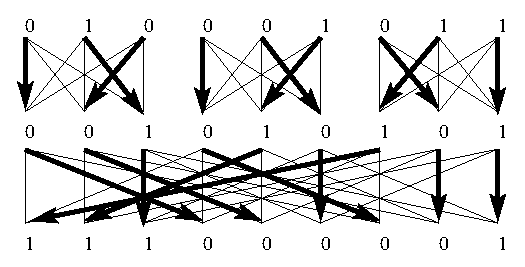
\includegraphics{radix3_network_2}}
\end{verbatim}
to include it as so:

\centerline{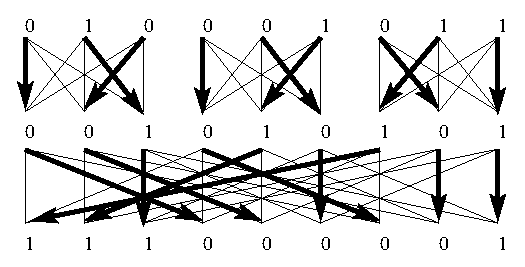
\includegraphics{radix3_network_2}}

Here, the \verb=\centerline= command centers the image on the line.  Be sure
to leave a blank line before and after this so it doesn't put it at the end or
beginning of a paragraph.

The \verb=\includegraphics= command also takes some optional arguments.  You
might find the \verb=scale= option to scale the image.  For example,
\begin{verbatim}
       \centerline{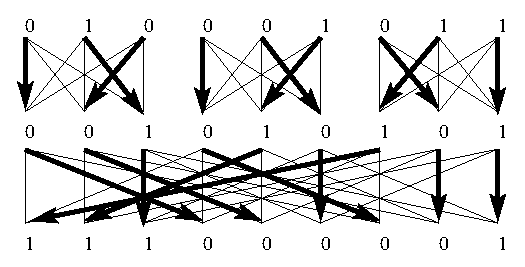
\includegraphics[scale=0.5]{radix3_network_2}}
\end{verbatim}
produces the following image that is scaled to half the original size.

\centerline{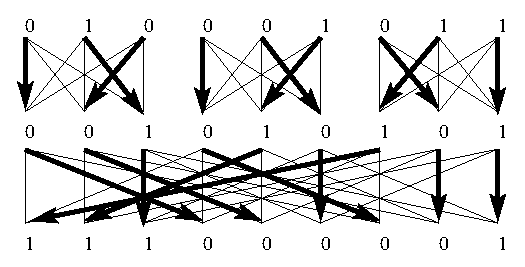
\includegraphics[scale=0.5]{radix3_network_2}}

You can also include more than one image on a line.  The commands 
\begin{verbatim}
        \centerline{
                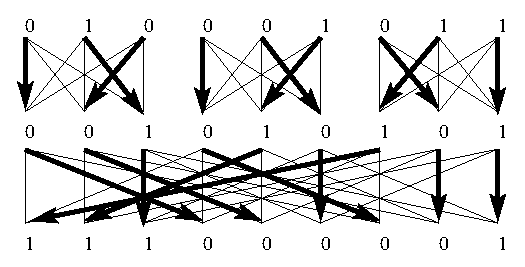
\includegraphics[scale=0.5]{radix3_network_2}
                \quad
                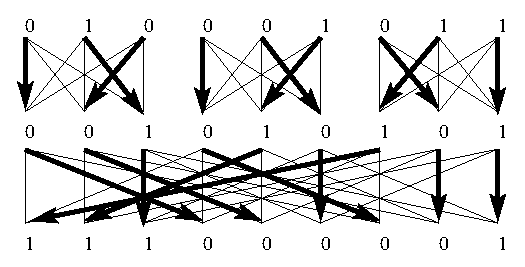
\includegraphics[scale=0.5]{radix3_network_2}
        }
\end{verbatim}
produces the following pair of images.  Here \verb=\quad= produces a little
spacing between the images.

\centerline{
        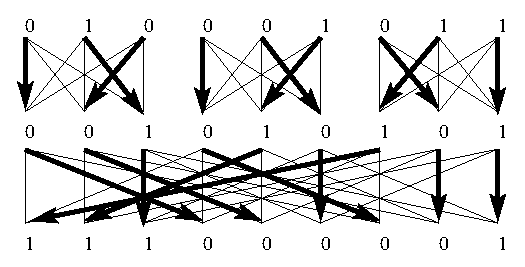
\includegraphics[scale=0.5]{radix3_network_2}
        \quad
        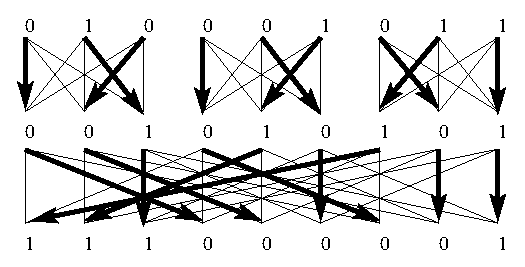
\includegraphics[scale=0.5]{radix3_network_2}
}


\subsection{Floating Environments}
\label{floats}

Unfortunately, image files are not smart enough to break to a new page, and
you may lose part of your image if  you place it too close to the end of a
page.  The solution is to use a \emph{floating environment} called the
\emph{figure} environment.  A floating environment floats to a convenient
location in the document.  You can specify where to allow the figure, and
\LaTeX{} will accommodate you as best it can.  For example, the text
\begin{verbatim}
        \begin{figure}[hbtp]
                \centerline{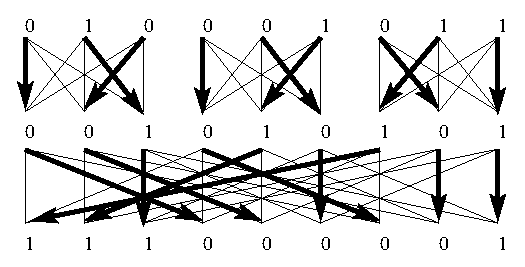
\includegraphics{radix3_network_2}}
                \caption{A test figure with the caption below.}
                \label{test fig}
        \end{figure}
\end{verbatim}
produces the Figure~\ref{test fig}.
\begin{figure}[hbtp]
        \centerline{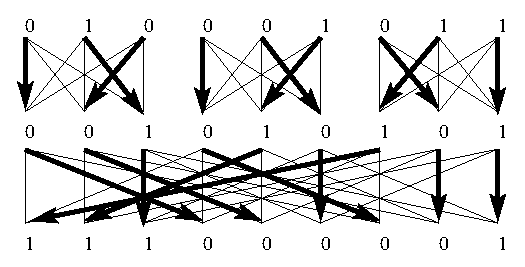
\includegraphics{radix3_network_2}}
        \caption{A test figure with the caption below.}
        \label{test fig}
\end{figure}

Here, the options \verb$[hbtp]$ tell \LaTeX{} to place the image \emph{here},
at the \emph{bottom} of the page, at the \emph{top} of the next page, or on a
\emph{page} of only images, in that order of preference.  You may remove some
of these designators if you want to limit where \LaTeX{} may place the image.

The \verb=\caption{...}= command places a caption on the figure.  It also
updates the figure counter, so be sure and place it before the
\verb=\label{...}= command.  By placing these commands at the end of the
figure environment, we tell \LaTeX{} to place the caption after the figure.
If you prefer, you can place these commands just after the
\verb=\begin{figure}= command to place the caption above the figure as in
Figure~\ref{test fig 2}.
\begin{figure}[hbtp]
        \caption{A test figure with the caption above.}
        \label{test fig 2}
        \centerline{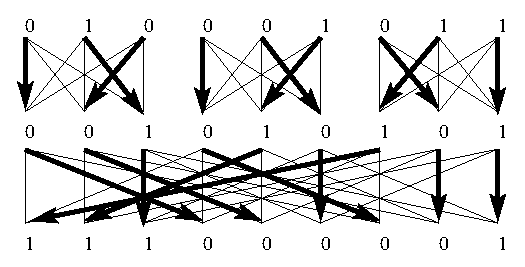
\includegraphics{radix3_network_2}}
\end{figure}

\LaTeX{} also has a \emph{table} environment for tables.

\subsection{Citations and the Bibliography}
\label{bib}

You may want to include a bibliography or list of references at the end of
your paper.  Happily, \LaTeX{} will help you automatically generate a
bibliography from a database file, called a \emph{BIB} file.  (For example,
Appendix~\ref{bib} has the \emph{BIB} file for this paper.)  This is another
plain text file that contains information about the sources you are using.  A
program called BibTeX takes the information from the database and includes
only the sources you cite.

In our document, we use the commands
\begin{verbatim}
        \bibliographystyle{plain}
        \bibliography{latex}
\end{verbatim}
to tell \LaTeX{} what form the bibliography should take and where to find the
content.  In this case, we are using the \emph{plain} style, which
alphabetizes the entries by author and typefaces them in a certain way.  A
different style might give a different typeface, a different method of
sorting, or both.

The \verb=\bibliography{latex}= tells \LaTeX to use the file \emph{latex.bib}
for the content information.  This command may take more than one argument
separated by commas.  For example, \verb=\bibliography{latex,foo}= tells
\LaTeX{} to also use the file \emph{foo.bib}

\subsubsection{\emph{BIB} Files}

The BIB file contains an entry for each reference, and each reference has a
corresponding type.  For example, the BIB file for this document contains
contains one book with the code
\begin{verbatim}
@Book{guide,
        author = "Helmut Kopka and Patrick W. Daly",
        title = "Guide to {LaTeX}",
        edition = "4th",
        publisher = "Pearson Education",
        address = "Upper Saddle River, NJ",
        year = 2003
}
\end{verbatim}
Here, \verb=guide= is the label we use for citing this reference.  It is
followed by several fields giving information about the book: its author,
title, edition, publisher, address, and year of publication.  Four of these
fields (author or editor, title, publisher, and year) are required, and the
others are optional.  We could also include fields for the volume or number,
series, month, and note \cite[Appendix B]{guide}.  Each field has a value
given by either a number--as the year--or a string in quotes.  Notice the
title contains \verb={LaTeX}= in the string.  This forces \LaTeX{} to use this
part of the string exactly as it appears instead of changing it to meet
whatever capitalization rules are specified in our particular bibliography
style.

Our BIB file also contains one journal article \cite{CEKSTV02}:
\begin{verbatim}
@Article{CEKSTV02,
        author =        "Li Chen 
                and Wayne Eberly 
                and Erich Kaltofen 
                and B. David Saunders 
                and William J. Turner
                and Gilles Villard",
        title = "Efficient Matrix Preconditioners for Black Box 
                Linear Algebra",
        journal =       "Linear Algebra and Applications",
        volume =        "343-344",
        pages = "119--146",
        note =  "Special issue on \emph{Infinite Systems of 
                Linear Equations Finitely Specified}, edited by 
                P. Dewilde, V. Olshevsky and A. H. Sayed",
        year =  2002,
        month = "March"
}
\end{verbatim}
This entry type requires four fields: author, title, journal, and year.  All
the other fields are optional.  Notice multiple authors are always separated
by the word ``and.''  This allows the BibTeX program to know how many authors
the paper has.

Our BIB file contains several entries for miscellaneous sources:
\begin{verbatim}
@Misc{tug,
        title = "{\TeX} Users Group web page",
        author = "{TeX Users Group}",
        howpublished = "Web page",
        note = "\url{http://www.tug.org}"
}
\end{verbatim}
These entry types actually requires no fields, but you may specify authors,
title, year, month, how published, and note.



\subsubsection{Citing Sources}

To cite a source, we use the \verb=\cite{...}= command.  For example, the
command \verb=\cite{CEKSTV02}= cites the article by Chen et al.
\cite{CEKSTV02}.  We can also use optional arguments to give a specific
location in the citation.  For example, the command
\verb=\cite[Theorem~6.1]{CEKSTV02}= cites Theorem 6.1 of the article by Chen
et al. \cite[Theorem 6.1]{CEKSTV02} and the command
\verb=\cite[Appendix~B]{guide}= cites Appendix B of the book by Kopka and Daly
\cite[Appendix B]{guide}.  We can also cite several sources at once as with
the command \verb=\cite{guide, CEKSTV02}=, which cites the \texttt{amsmath}
user's guide and the AMS-\LaTeX{} website \cite{guide, CEKSTV02}.

\subsubsection{BibTeX}

Once you have created a BIB file and cited some sources, you can use the
BibTeX program to create a bibliography.  To do so, place the
\verb=\bibliography{...}= command where you want the bibliography to appear
and place the command \verb=\bibliographystyle{...}= anywhere before it.
Then typeset the file once with \LaTeX{}.  Finally run \emph{BibTeX} from the
\emph{Tools} menu and \LaTeX{} the file again at least once or twice more.

\subsubsection{Author-Year Bibliographies with \text{natbib}}

The standard \LaTeX{} bibliography implementation numbers references and cites
them by their numbers.  An alternative style that many journals and texts use
references works by citing the author's name and year of publication.  This
may take the familiar form of the APA style that many standard English style
guides include, or other related forms.  There are a number of packages
developed to deal with this situation, but the most universal of these is the
\texttt{natbib} package by Patrick W. Daly.  It is compatible with the standard
bibliography styles as well as a number of author-year styles.  See \S 11.3.4
of the \emph{Guide to LaTeX} by Helmut Kopka and Patrick W. Daly \cite{guide}
for more information. 

\section{More Information}
\label{more}

You can easily find more information about \LaTeX{}.  The \TeX{} Users Group
maintains a website \cite{tug} that contains links to all the information you
might ever want to know about \TeX{} and \LaTeX{}.  You can find information
about obtaining freeware and commercial software for any computer platform,
tutorials and documents describing how to do anything you'd ever want to do,
and books about \TeX{} and \LaTeX{}.  If you are interested in a good book
about \LaTeX{}, check out the book \emph{Guide to LaTeX} by Helmut Kopka and
Patrick W. Daly \cite{guide}.

\bibliographystyle{plain}
\bibliography{latex}

%% \newpage
%% \part*{Appendices}
\appendix

%% \section{Raw \LaTeX{} input}
%% \label{input}
%% 
%% \begin{small}
%%         \verbatiminput{latex.tex}
%% \end{small}

%% \section{Bibliographic Database}
%% \label{bib input}
%% 
%% \begin{small}
%%         \verbatiminput{latex.bib}
%% \end{small}

\section{Mathematical Symbols}
\label{symbols}

The following tables give some of the basic mathematical symbols you might
want to use.  They demonstrate some of the symbols normally accessible from
\emph{math mode}.  You can consult other \LaTeX{} references for more symbols.
In particular, Oetiker~\cite{lshort} and Kopka and Daly~\cite{guide} provide
tables of mathematical symbols.  Perkins~\cite{symbols} provides one of the
most comprehensive symbol lists available.

%%%%%%%%%%%%%%%%%%%%%%%%%%%%%%%%%%%%%%%%%%%%%%%%%%%%%%%%%%%%%%%%%
% Contents: TeX and LaTeX and AMS symbols for Maths
% $Id: lssym.tex,v 1.2 2003/03/19 20:57:46 oetiker Exp $
%%%%%%%%%%%%%%%%%%%%%%%%%%%%%%%%%%%%%%%%%%%%%%%%%%%%%%%%%%%%%%%%%

%
%
% Symbol Entry for Math Symbol Tables
%
\newcommand{\X}[1]{$#1$&\texttt{\string#1}\hspace*{1ex}}
% normal text .... 
\newcommand{\SC}[1]{#1&\texttt{\string#1}\hspace*{1ex}}
% for accents in text mode
\newcommand{\A}[1]{#1&\texttt{\string#1}\hspace*{1ex}}
\newcommand{\B}[2]{#1#2&\texttt{\string#1{} #2}\hspace*{1ex}}

\newcommand{\W}[2]{$#1{#2}$&
  \texttt{\string#1}\texttt{\string{\string#2\string}}\hspace*{1ex}}
\newcommand{\Y}[1]{$\big#1$ &\texttt{\string#1}}  %
\newcommand{\Z}[1]{\texttt{\string#1}}  %
% Mathsymbol Table
\newsavebox{\symbbox}
\newenvironment{symbols}[1]%
{\par\vspace*{2ex}
\renewcommand{\arraystretch}{1.1}
\begin{lrbox}{\symbbox}
\hspace*{4ex}\begin{tabular}{@{}#1@{}}}%
{\end{tabular}\end{lrbox}\makebox[\textwidth]{\usebox{\symbbox}}\par\medskip}


\begin{table}[!h]
\caption{Math Mode Accents.}  \label{mathacc}
\begin{symbols}{*4{cl}}
\W{\hat}{a}     & \W{\check}{a} & \W{\tilde}{a} & \W{\acute}{a} \\
\W{\grave}{a} & \W{\dot}{a} & \W{\ddot}{a}    & \W{\breve}{a} \\
\W{\bar}{a} &\W{\vec}{a} &\W{\widehat}{A}&\W{\widetilde}{A}\\  
\end{symbols}
\end{table}
 
\begin{table}[!h]
\caption{Greek Letters.}
\begin{symbols}{*4{cl}}
 \X{\alpha}     & \X{\theta}     & \X{o}          & \X{\upsilon}  \\
 \X{\beta}      & \X{\vartheta}  & \X{\pi}        & \X{\phi}      \\
 \X{\gamma}     & \X{\iota}      & \X{\varpi}     & \X{\varphi}   \\
 \X{\delta}     & \X{\kappa}     & \X{\rho}       & \X{\chi}      \\
 \X{\epsilon}   & \X{\lambda}    & \X{\varrho}    & \X{\psi}      \\
 \X{\varepsilon}& \X{\mu}        & \X{\sigma}     & \X{\omega}    \\
 \X{\zeta}      & \X{\nu}        & \X{\varsigma}  & &             \\
 \X{\eta}       & \X{\xi}        & \X{\tau} 
\end{symbols}

\begin{symbols}{*4{cl}}
 \X{\Gamma}     & \X{\Lambda}    & \X{\Sigma}     & \X{\Psi}      \\
 \X{\Delta}     & \X{\Xi}        & \X{\Upsilon}   & \X{\Omega}    \\
 \X{\Theta}     & \X{\Pi}        & \X{\Phi} 
\end{symbols}
\end{table}

\begin{table}[!tbp]
\caption{Binary Relations and Operators.}\label{tab:binary}
You can negate the following symbols by prefixing them with a \verb=\not= command.  
%However, \verb=\not\mid= produces the symbol $\not\mid$.  For better results, use the \texttt{amssymb} package and the \verb=\nmid= command to produce $\nmid$.
The \verb=\nmid= command requires the \texttt{amssymb} package.
\begin{symbols}{*3{cl}}
 \X{<}           & \X{>}           & \X{=}         \\
 \X{\leq}or \verb|\le|   & \X{\geq}or \verb|\ge|   & \X{\neq}or \verb|\ne| \\
 \X{\ll}         & \X{\gg}         & \X{\equiv}     \\
 \X{\subset}     & \X{\supset}     & \X{\approx}    \\
 \X{\subseteq}   & \X{\supseteq}   & \X{\cong}      \\
 \X{\in}         & \X{\ni}, \verb|\owns|  & \X{\notin} \\
 \X{\mid}        & \X{\nmid}       & \X{\parallel}   \\
 \X{\perp}       & \X{:}           & \X{\propto}    \\
\end{symbols}

\begin{symbols}{*3{cl}}
 \X{+}              & \X{-}              & \X{\circ}         \\
 \X{\pm}            & \X{\mp}            & \X{\ast}          \\
 \X{\cdot}          & \X{\div}           & \X{\bullet}       \\
 \X{\times}         & \X{\setminus}      & \X{\dagger}       \\
 \X{\cup}           & \X{\cap}           & \X{\ddagger}      \\
 \X{\vee}, \verb|\lor|     & \X{\wedge}, \verb|\land|  
\end{symbols}
 
\end{table}

\begin{table}[!tbp]
\caption{Variable-Sized Operators.}
\begin{symbols}{*4{cl}}
 \X{\sum}      & \X{\bigcup}   & \X{\bigvee}   & \\
 \X{\prod}     & \X{\bigcap}   & \X{\bigwedge} &\\
 \X{\int}      & \X{\oint}     & &             & 
\end{symbols}
 
\end{table}


\begin{table}[!tbp]
\caption{Arrows.}
\begin{symbols}{*3{cl}}
 \X{\leftarrow}or \verb|\gets|& \X{\longleftarrow} & \X{\uparrow}          \\
 \X{\rightarrow}or \verb|\to|& \X{\longrightarrow} & \X{\downarrow}        \\
 \X{\leftrightarrow}    & \X{\longleftrightarrow}& \X{\updownarrow}      \\
 \X{\Leftarrow}         & \X{\Longleftarrow}     & \X{\Uparrow}          \\
 \X{\Rightarrow}        & \X{\Longrightarrow}    & \X{\Downarrow}        \\
 \X{\Leftrightarrow}    & \X{\Longleftrightarrow}& \X{\Updownarrow}      \\
 \X{\mapsto}            & \X{\longmapsto}        & \\
 \X{\iff}(bigger spaces)& 

\end{symbols}
\end{table}

\begin{table}[!tbp]
\caption{Log-like Symbols.}\label{tab:log-like}
\begin{symbols}{*8{cl}}
\Z\arccos & \Z\cos  & \Z\coth & \Z\det & \Z\gcd & \Z\ln     & \Z\min & \Z\sinh \\
\Z\arcsin & \Z\cosh & \Z\csc & \Z\dim & \Z\lim  & \Z\log    & \Z\sec & \Z\tan  \\
\Z\arctan & \Z\cot  & \Z\deg & \Z\exp & \Z\lg   & \Z\max    & \Z\sin & \Z\tanh \\
\end{symbols}

{\centering\footnotesize
  Calling the above ``symbols'' may be a bit misleading.
  Each log-like symbol merely produces the eponymous textual equivalent,
  but with proper surrounding spacing.}
\end{table}

\begin{table}[!tbp]
\caption{Delimiters.}\label{tab:delimiters}
\begin{symbols}{*4{cl}}
 \X{(}            & \X{)}            & \X{\uparrow} & \X{\Uparrow}    \\
 \X{[}or \verb|\lbrack|   & \X{]}or \verb|\rbrack|  & \X{\downarrow}   & \X{\Downarrow}  \\
 \X{\{}or \verb|\lbrace|  & \X{\}}or \verb|\rbrace|  & \X{\updownarrow} & \X{\Updownarrow}\\
 \X{\langle}      & \X{\rangle}  & \X{|}or \verb|\vert| &\X{\|}or \verb|\Vert|\\
 \X{\lfloor}      & \X{\rfloor}      & \X{\lceil}       & \X{\rceil}      \\
 \X{/}            & \X{\backslash}   & &. (dual. empty)
\end{symbols}
\end{table}

\begin{table}[!tbp]
\caption{Miscellaneous Symbols.}
\begin{symbols}{*4{cl}}
 \X{\dots}       & \X{\cdots}      & \X{\vdots}      & \X{\ddots}     \\
 \X{\infty}      & \X{\imath}      & \X{\jmath}      & \X{\ell}       \\
 \X{\forall}     & \X{\exists}     & \X{\partial}    & \X{\nabla}     \\
 \X{'}           & \X{\prime}      & \X{\emptyset}   & \X{\angle}     \\
\end{symbols}
\end{table}

\begin{table}[!tbp]
\caption{Non-Mathematical Symbols.}
\bigskip
These symbols can also be used in text mode.
\begin{symbols}{*4{cl}}
 \SC{\dag}  &  \SC{\S}  &  \SC{\copyright} &  \SC{\textregistered}  \\
 \SC{\ddag} &  \SC{\P}  &  \SC{\pounds}    &  \SC{\%}               \\
\end{symbols}
\end{table}

\begin{table}[!tbp]
\caption{Math Alphabets.}
\begin{symbols}{@{}*3l@{}}
Example& Command &Required package\\
\hline
\rule{0pt}{1.05em}$\mathrm{ABCDE abcde 1234}$
        & \verb|\mathrm{ABCDE abcde 1234}|
        &       \\
$\mathit{ABCDE abcde 1234}$
        & \verb|\mathit{ABCDE abcde 1234}|
        &       \\
$\mathnormal{ABCDE abcde 1234}$
        & \verb|\mathnormal{ABCDE abcde 1234}|
        &  \\
$\mathcal{ABCDE}$
        & \verb|\mathcal{ABCDE}|
        &  \\
%% $\mathscr{ABCDE}$
%%        &\verb|\mathscr{ABCDE}|
%%        &\emph{mathrsfs}\\
$\mathfrak{ABCDE abcde 1234}$
        & \verb|\mathfrak{ABCDE abcde 1234}|
        &\emph{amsfonts}  or \emph{amssymb}  \\
$\mathbb{ABCDE}$
        & \verb|\mathbb{ABCDE}|
        &\emph{amsfonts}  or \emph{amssymb} \\
\end{symbols}
\end{table}



\end{document}
